% 1961 年全国卷第 5 题：排水管圆截面中的水弓形。
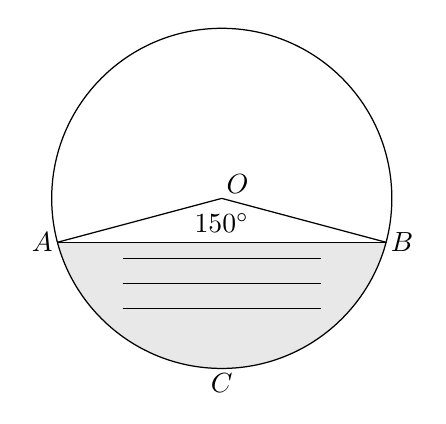
\begin{tikzpicture}[scale=0.9, line width=0.45pt,
  every node/.style={inner sep=1.5pt}]
  \coordinate (O) at (0,0);
  \coordinate (A) at (-2.32,-0.62);
  \coordinate (B) at (2.32,-0.62);
  \fill[gray!18] (A) arc (195:345:2.4) -- cycle;
  \draw (O) circle (2.4);
  \draw (A)--(B);
  \draw (O)--(A) (O)--(B);
  \foreach \y in {-1.55,-1.2,-0.85} {
    \draw (-1.4,\y)--(1.4,\y);
  }
  \node[anchor=east] at (A) {$A$};
  \node[anchor=west] at (B) {$B$};
  \node[anchor=south west] at (O) {$O$};
  \node at (0,-0.35) {$150^\circ$};
  \node[anchor=north] at (0,-2.4) {$C$};
\end{tikzpicture}
